\subsubsection{Flow Engineering}
\label{mazu-floweng}

\begin{figure}
\centering
  \centering
  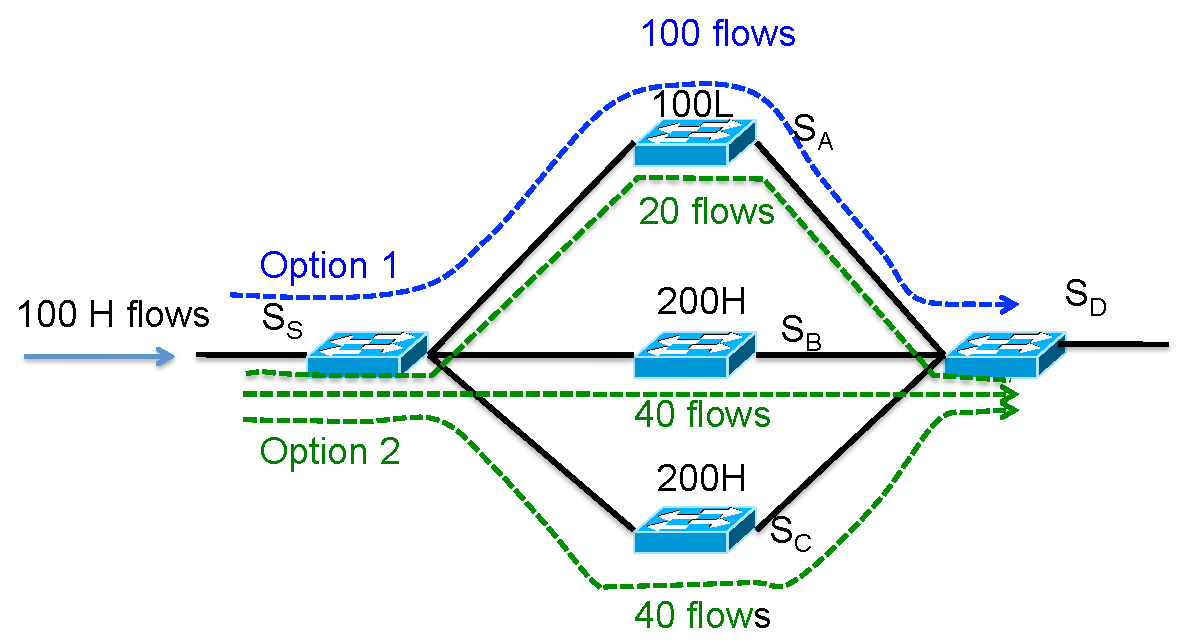
\includegraphics[width=0.55\textwidth]{figures/mazu/flow_eng_example.pdf} 
\caption{Flow 
engineering example, assuming \BroadcomOne. $nL$ = $n$ low priority rules;
$nH$ = $n$ high priority rules; capacity = 1000 rules. Ingress and egress 
tables are empty} 
\label{fig:flow_eng} 
\end{figure}

SDN applications that perform failure recovery, traffic engineering, or other
forms of routing must quickly compute and setup network paths in order to
satisfy reachability and performance objectives. These applications must often
select one of many possible paths based on congestion, delay, flow table 
occupancy, or other metrics. Unfortunately, a (slightly) more optimal path 
according to these metrics may take significantly longer to setup due to 
outbound latency.

For example, consider an SDN application that seeks to minimize the
imbalance in flow table occupancy~\cite{hong2013achieving, qazi2013simple, moshref2013vcrib}. If such an
application needed to setup routes for 100 flows of high priority $H$ in the
topology shown in Figure~\ref{fig:flow_eng}, it would select the first path
through switch $S_A$ for all flows, thereby equalizing the number of flow
table entries across all switches. However, assuming the switches are
\BroadcomOne, this would require displacing {\em each} of the 100 existing
rules of low priority $L$ in $S_A$ for {\em each} of the 100 new flows,
resulting in a total flow installation time of $\approx$1.5s. In contrast, by
routing only 20 new flows through $S_A$, and dividing the remaining flows
evenly between the paths through $S_B$ and $S_C$, we can keep the same level
of imbalance in flow table occupancy ($S_B$ and $S_C$ each have twice as many
entries as $S_A$), while reducing the total flow installation time to
$\approx$0.3s (assuming rules are installed in $S_A$, $S_B$, and $S_C$ in
parallel). 


The goal of {\em flow engineering} (\FE) is to select paths that minimize
installation delay while still satisfying an SDN application's primary path
selection criteria (e.g., flow table occupancy or congestion). Assuming there
are many possible sets of paths $\{\mathcal{P}^i_{obj}\}_i$ that (closely)
satisfy an application's objectives, FE selects the set
$\mathcal{P}^{displace}_{obj,tbl\_sz}$ that minimizes the aggregate
latency impact of rule installations, and any associated rule displacements,
while still obeying flow table space constraints.
$\mathcal{P}^{displace}_{obj,tbl\_sz}$ can be computed using a two step
optimization:
({\em i}) identify sets of paths that satisfy the SDN application's objective 
function,
but do not select the actual
paths to use; ({\em ii}) select paths that minimize aggregate
flow installation time.
Unfortunately, the time required to solve the integer linear program would
outweigh the latency benefits it seeks provide, so we formulate an
efficient heuristic.

\tightparagraph{Flow Engineering Heuristic}
Our goal is to satisfy a bound $C$ on the time required to install/modify
rules across all switches. 

We represent the network as a graph $G = (V,E)$, where each node is a switch
(or PoP) and each edge is a link (or tunnel). Given a traffic matrix $M$, the
SDN application computes $K$ candidate equal cost paths for each $(u,v) \in
V$, where cost is defined in terms of the application's objective (e.g.,
average link utilization). We assume the application also assigns a priority
$Pri(u,v)$ to each flow $(u,v)$.


We sort the flows in decreasing order of resource demand (e.g., bandwidth) and
iterate through them. For each flow $(u,v)$ in the sorted order, we consider
the corresponding $K$ equal cost paths in decreasing order of resource 
availability; let $P^{1\ldots K}_{(u,v)}$ be the sorted order. If the resource
demand $d_{uv}$ can be satisfied by the path $P^{1}_{(u,v)}$, then we compute
whether installing/updating rules for flow $(u,v)$ along this path violates the
latency bound $C$.

Given our measurement results, for every switch $s \in P^{1}_{(u,v)}$, we can
model the latency at $s$ due to installing rules for $(u,v)$ as 
$L_s = \max(a, (b +c * Disp_s(Pri(u,v))))$. Here, $Disp_s(Pri(u,v))$ is the 
number of rules at $s$ that will be displaced by the rule for $(u,v)$.
$a$, $b$ and $c$ are constants derived from switch
measurements. This model essentially says that if the current rule
does not displace any rules from $s$'s existing table, then it incurs
a fixed cost of $a$; otherwise, it incurs the cost given by $b +c *
Disp_s(Pri(u,v))$. The fixed cost $a$ is the insertion delay without any TCAM
reordering. 

Now, $\forall s \in P^{1}_{(u,v)}$, we check if $L_s + CurrentL_s \le C$,
where $CurrentL_s$ is the current running total cost of installing the
rules at $s$, accumulated from vertex pairs considered prior to $(u,v)$ in our
iterative approach.
If this inequality is satisfied, we assign $(u,v)$ to the path
$P^{1}_{(u,v)}$ and move to the next vertex pair. If not,
we move to the next candidate path for $(u,v)$, i.e., $P^{2}_{(u,v)}$ and
repeat the process.
If after iterating through all flows once, we have not selected a feasible
path for each flow, then we increase $C$ and start from the beginning.
Alternately, we could do a simple binary search on $C$. 

\tightparagraph{Limitations} Because paths are computed by the SDN application, FE
must be integrated with the application. FE does not apply to scenarios where 
route updates are confined to a single location, presenting no opportunity to
spread update load laterally. One such example is MicroTE~\cite{benson2011microte},
where changes in traffic demands are accommodated by altering rules at the
source ToR to reallocate ToR-to-ToR flows across different tunnels.

